%% Tex spellcheck = fr_FR
\chapter{Chapter 3 : GPS Overview}

In this chapter, we will explore the \gls{gps} system, its history, its architecture, the technologies involved, the signals it uses. We will explore the different frequency bands and codes used by the system. However the actual explanation of how the system actually works will be done in the next chapters.

\section{Brief history}

The \gls{gps} system was developed by the United States Department of Defense and became fully operational in 1995. It was created to provide a precise and continuous navigation system for the military. The system was opened to civilian use in the 1980s and has since become a global utility. It was the first \gls{gnss} to be developed and is still the most widely used and supported by the majority of devices.

\section{System architecture}

The \gls{gps} system consists of three segments:
\begin{itemize}
	\item The user segment
	\item The space segment
	\item The control segment
\end{itemize}


\subsection{User segment}

The user segment is composed of the receivers that are used to determine the position, velocity and time. These receivers are used in a wide variety of applications, including aviation, agriculture, construction, maritime, mining, public safety, transportation, etc.

\newpage

\subsection{Control segment}

The control segment \footcite{noauthor_gpsgov_nodate} is composed of a network of ground facilities that are used to monitor and control the \gls{gps} satellites. These facilities are used to track the satellites, upload updated navigation data, and ensure the overall health of the satellite constellation. They might

\begin{figure}[H]
	\centering
	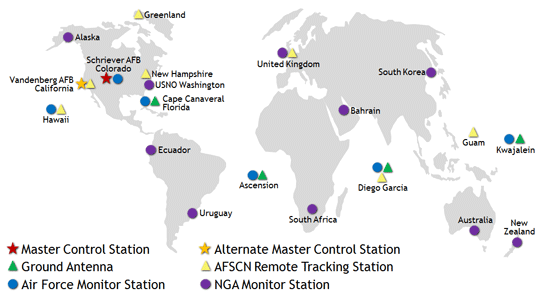
\includegraphics[width=1\linewidth]{gps_control_segment.png}
	\caption[GPS Control segment]{World map of ground facilities of the Control segment of GPS Source: www.gps.gov ref: URL04}
	\label{fig:gps_control_segment}
\end{figure}

\subsection{Space segment}

The Space segment \footcite{noauthor_gpsgov_nodate} is composed of a constellation of 31 operational sattelites as of 15 Auguest 2023 \footcite{noauthor_list_2024}. Each of these satellite (\gls{sv}) is in a \gls{meo} at an altitude of approximately 20,200 km. These satellites are arranged into six equally-spaced orbital planes, with an inclination of 55 degrees in relation to the equator.

\begin{figure}[H]
	\centering
	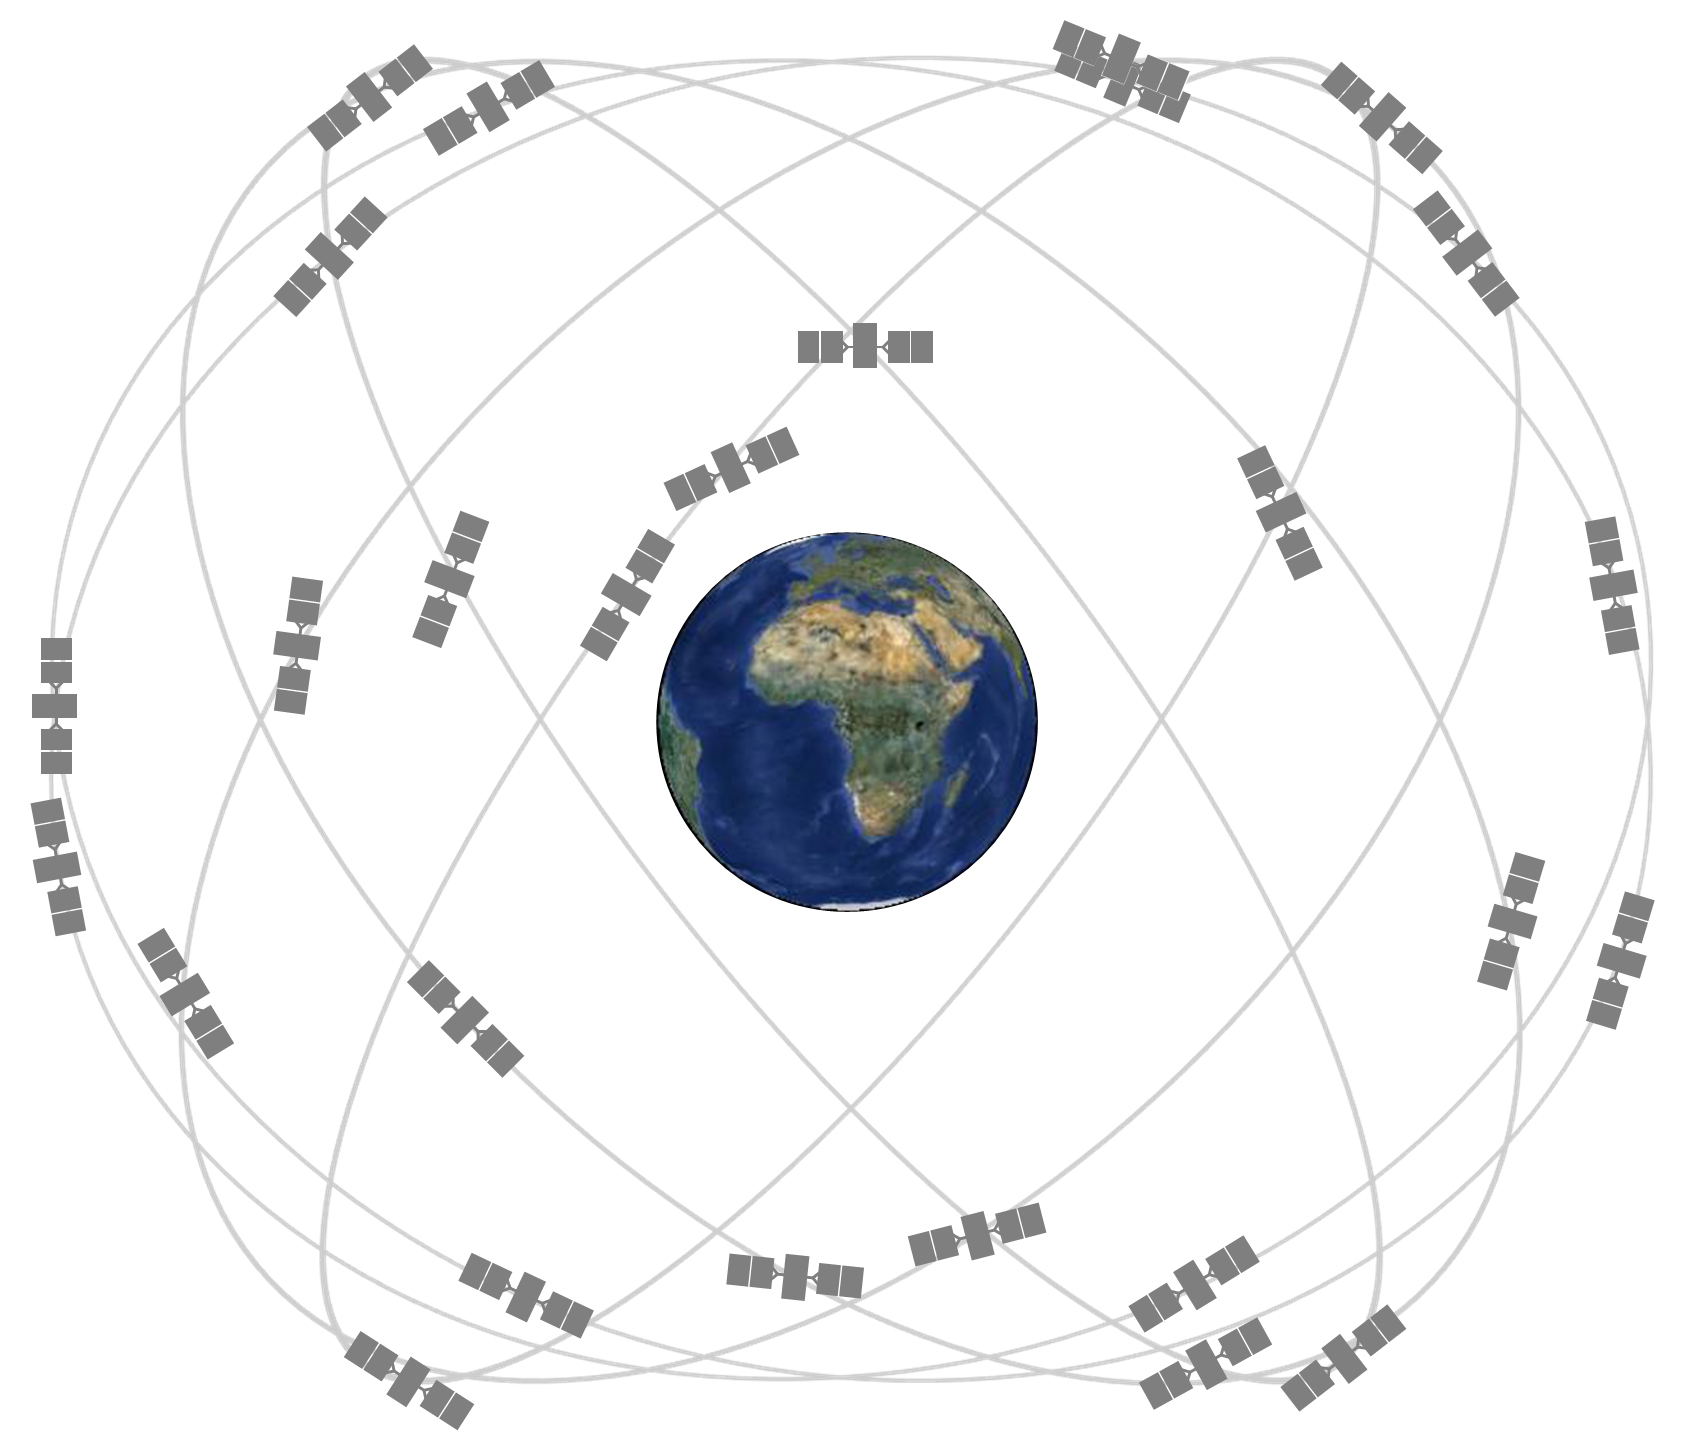
\includegraphics[width=0.5\linewidth]{gps_constellation.jpg}
	\caption[GPS Satellite constellation]{GPS constellation Source:www.gps.gov ref: URL01}
	\label{fig:gps_constellation}
\end{figure}

\begin{figure}[H]
	\centering
	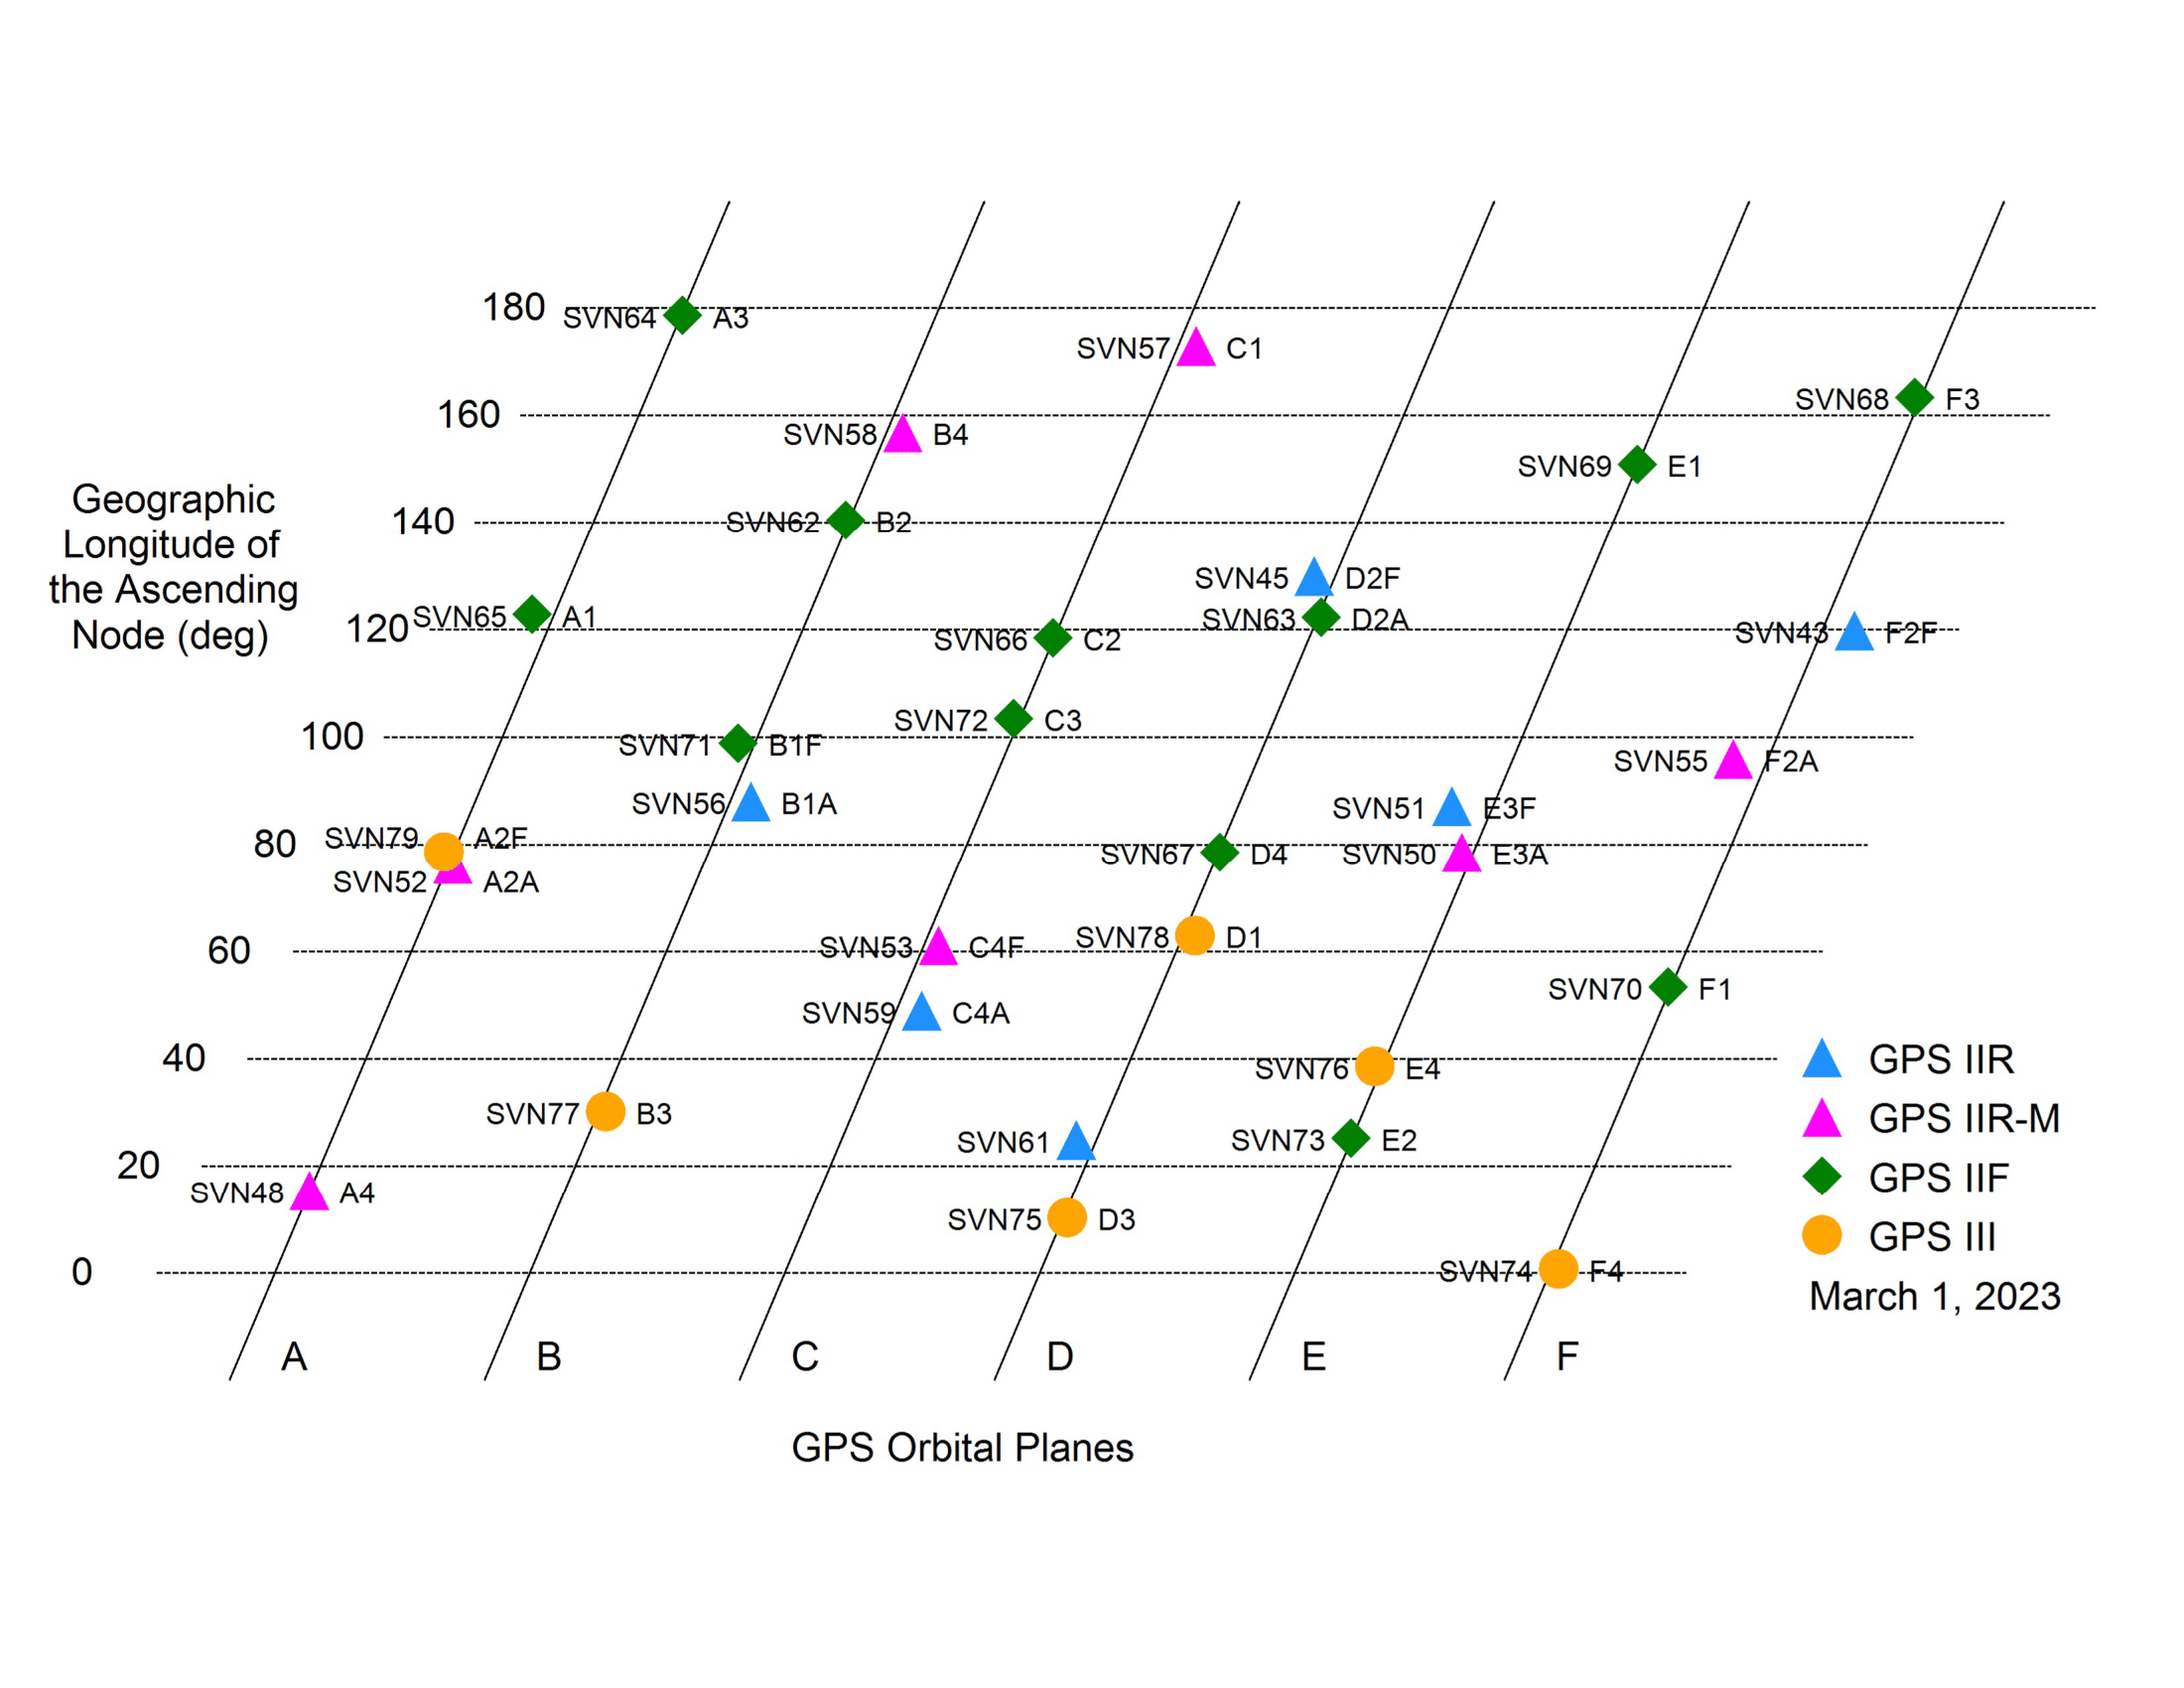
\includegraphics[width=0.8\linewidth]{gps_planes.png}
	\caption[GPS Orbital planes]{GPS Orbital planes Source:www.navcen.uscg.gov ref: URL02}
	\label{fig:gps_planes}
\end{figure}

Each of these \gls{sv} are placed in a Sub-Geostationary orbit, making them rotate two times a around earth each day. These \gls{sv} are placed in such a way that at any time, anywhere on Earth, there are at least \textbf{six} of them visible with an average of \textbf{nine} visible in the sky. Note that these numbers are acheived with the current constellation, but a minimum constellation of 24 sattelites is required for the system to work.

There have been five main satellite models developed for the \gls{gps} system, each with different capabilities and improvements over the previous

\begin{figure}[H]
	\centering
	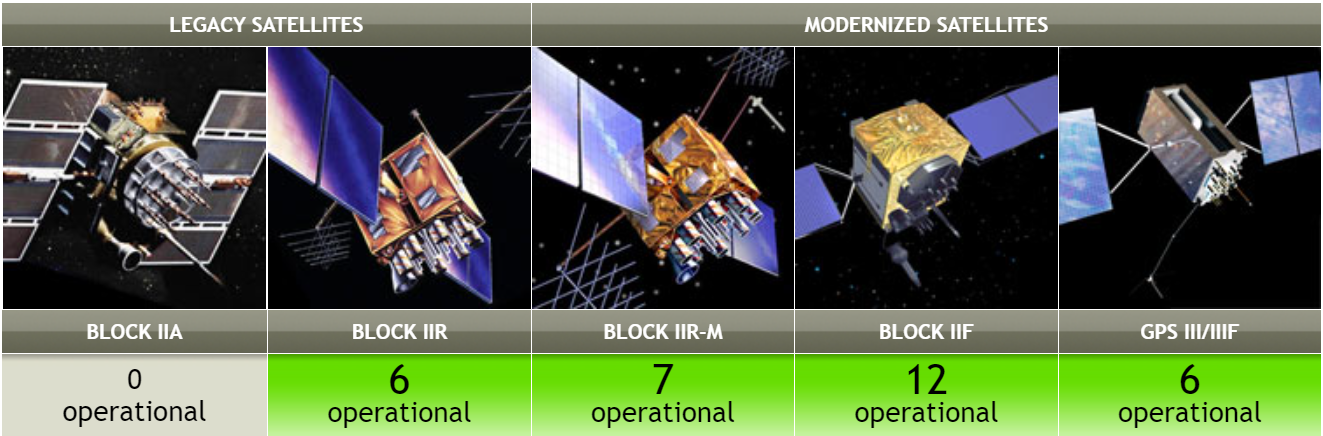
\includegraphics[width=1\linewidth]{gps_satellites.png}
	\caption[GPS Satellites generations]{Current and Future Satellite Generations Source: www.gps.gov ref: URL03}
	\label{fig:gps_satellites}
\end{figure}

\pagebreak

\section{Basic GPS principle}

The \gls{gps} constellation broadcasts signals constantly to the Earth. These signals are used by receivers to determine a position, velocity and time. Time is given as a direct value but position is computed using a process called \textbf{trilateration}. This process is based on the time it takes for the signals to travel from the satellites to the receiver and the known position of the satellites (Given in the broadcast messages). We'll explain things from a single bit data to the frames messages to the end user position.
% TODO: CITE NEXT


\section{Satellite hardware}

Each \gls{gps} satellite is equipped with \textbf{four} atomic clocks, two rubidium and two cesium. These atomic clocks allow us to generate a \textbf{Fondamental Frequency} ($ F0 $) of 10.23 MHz. This frequency is then multiplied to generate the \textbf{L1}, \textbf{L2} and \textbf{L5} frequencies.


\section{Signals and frequencies}

\subsection{Frequency bands}

As mentionned earlier, the \gls{gps} system broadcasts three signals, each on a different frequency band. These bands are \textbf{L1}, \textbf{L2} and \textbf{L5}.
% List
\begin{itemize}
	\item The \textbf{L1} band, centered at \textbf{1575.42} MHz ($F = 154 \cdot F0 $).
	\item The \textbf{L2} band, centered at \textbf{1227.60} MHz ($F = 120 \cdot F0 $).
	\item The \textbf{L5} band, centered at \textbf{1176.45} MHz ($F = 115 \cdot F0 $).
\end{itemize}

\subsection{L1 Codes}

Four different codes are sent on the \textbf{L1} band, two of them are used for civilian use, the \textbf{C/A} and \textbf{P(Y)} (Precision) codes.
One of them is reserved for the military, the \textbf{M-code}.
The last one is an evolution of the L1 signal : the \textbf{L1C}. This signal is designed to be interoperable with other \gls{gnss} systems like Galileo.


\subsection{L2 Codes}

The \textbf{L2} band is used to send two different code, the \textbf{L2 CM} and the \textbf{L2 CL} codes. These are mostly used for dual-frequency receivers to remove the ionospheric delay. This works by taking the difference between the two signals and by knowing the actual speed of each frequency in the same medium.

\subsection{L5 Codes}

The \textbf{L5} band is the third civilian signal \footcite{noauthor_gps_nodate}, it has been introduced to meet demanding requirements for safety-of-life transportation. It is provided as a future proof signal for aviation use. Combined with the \gls{ca} code, it provides accuracy and robustness via ionospheric correction and redundancy.

This code is given as a new way for aviation to increase capacity and fuel efficiency within \gls{usa} airspace, railroads, highways and waterways.


\section{PRN code generation}

Each satellite sending gls{ca} code is allocated a unique \gls{prn} code, this code is used to identify the satellite and to allow the receiver to distinguish between the signals of different satellites. The \gls{prn} code is a \textbf{Gold code} that is generated by a \textbf{Linear Feedback Shift Register} (LFSR). This code is a pseudo-random sequence of 1023 bits that repeats every millisecond. This code is then modulated with the carrier frequency to generate the signal that is broadcasted by the satellite.

Each \gls{sv} is assigned a unique identifier from which a \gls{prn} can be generated. As explained in \ref{fig:prn_generator} figure, each ID is correspond to a pair of "taps", these taps are the bit positions in the polynomial generator. There is 2 polynomial generator, used together to generate the \gls{prn} code.

The generated codes are \textbf{Gold codes} or \textbf{Gold sequences} so they have a small cross-correlation between them. This means that the receiver can easily distinguish between the signals of different satellites.

\begin{figure}[H]
	\centering
	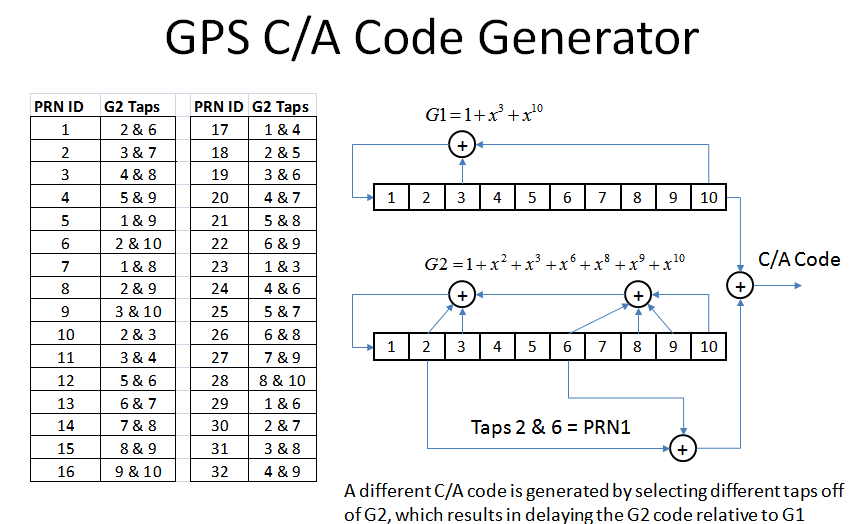
\includegraphics[width=1\linewidth]{prn_generator.png}
	\caption[PRN code generators]{PRN code generators Source: https://i.stack.imgur.com ref: URL013}
	\label{fig:prn_generator}
\end{figure}



%\begin{figure}[tbph!]
%	\centering
%	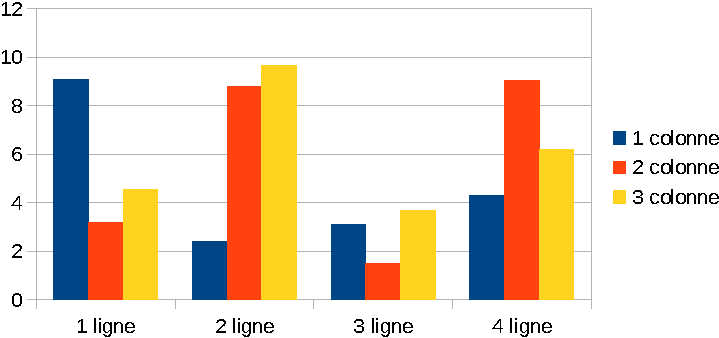
\includegraphics[width=0.7\linewidth]{chart}
%	\caption[Diagramme Truc.]{Diagramme Truc. Source: rapport d'activité 2019 de MonEntrepriseDeStage.}
%	\label{fig:chart3}
%\end{figure}